% PREAMBLE
\documentclass[a4paper, 12pt, oneside]{article}
\linespread{1.5} %space between lines

\pagestyle{plain}

\usepackage{geometry} %margins
\geometry{a4paper, top=3cm, bottom=3cm, left=3cm, right=3cm, bindingoffset=5mm}


\usepackage{multicol} % multi columns
\usepackage{ragged2e} % text alignment
\usepackage{lmodern} % use modern font style

\usepackage{listings}
\lstset{frame=tb, % listings config, this can be changed in the document body as well
  language=bash,
  aboveskip=3mm,
  belowskip=3mm,
  showstringspaces=false,
  columns=flexible,
  basicstyle={\small\ttfamily},
  numbers=none,
  numberstyle=\tiny\color{SpringGreen},
  keywordstyle=\color{NavyBlue},
  commentstyle=\color{gray},
  stringstyle=\color{Orange},
  breaklines=true,
  breakatwhitespace=true,
  tabsize=3,
  captionpos=b
}

\usepackage{amsmath}
\usepackage[english]{babel} % main language
\usepackage{csquotes}
\usepackage[labelfont=bf]{caption}
\usepackage[backend=biber, style=nature]{biblatex} % bibliography
\addbibresource{biblio.bib}

\usepackage{comment}
\usepackage{xpatch}
\usepackage{blindtext}

\makeatletter

\xpatchcmd{\@makeschapterhead}{%
  \Huge\bfseries  #1\par\nobreak%
}{%
  \Huge \bfseries\centering #1\par\nobreak%
}{\typeout{Patched makeschapterhead}}{\typeout{patching of @makeschapterhead failed}}


\xpatchcmd{\@makechapterhead}{%
  \huge\bfseries \@chapapp\space \thechapter
}{%
  \huge\bfseries\centering \@chapapp\space \thechapter
}{\typeout{Patched @makechapterhead}}{\typeout{Patching of @makechapterhead failed}}

\makeatother

\usepackage{fancyhdr}
\usepackage[export]{adjustbox}

\usepackage{hyperref} % hyperlink
\hypersetup{
    colorlinks=true,
    citecolor=teal,
    linkcolor=black,
    urlcolor=black,
    pdftitle=Master Thesis,
    pdfauthor=Mattia Toninelli,
    }

\usepackage{booktabs}
\usepackage{multirow}
\usepackage[table,xcdraw,dvipsnames]{xcolor}
\usepackage{graphicx}
\graphicspath{ {./figures/} }

\usepackage{lscape}
\usepackage{float}
\usepackage{wrapfig}
% PREAMBLE END

%DOCUMENT START
\begin{document}
\begin{titlepage} % change \vspace{} values for the desired results

  \begin{center}
    
\includegraphics{images/logo.jpg}\par
    \vspace{1cm}
    {\scshape\large GPU Computing Project\par}
    \vspace{4cm}
    {\scshape\large\bfseries Bitonic Sort using Numba on NVIDIA GPUs\par}
    \vspace{4cm}
  \end{center}

  \begin{center}
    \scshape\normalsize\textbf{Author:}\\Manuele Lucchi\\08659A \par
  \end{center}

  \vfill

  % Bottom of the page
  {\begin{center}
      \scshape\large Academic Year 2022/2023
    \end{center}}

\end{titlepage}

\section{Abstract}
This documents describe the performances of an existing algorithm, the Bitonic Sort, implemented using Python and Numba, comparing it with a serial approach and CUDA C implementation.

\tableofcontents

\section{Introduction}
The Bitonic Mergesort \cite{bitonic} is an algorithm created in 1968 by Ken Batcher\cite{ken}. The elements to choose for the comparison are indipendent from the value (it's not data-dependant) therefore is well suited for parallel processing.\\
Over the years there are been many implementations using low level languages such as C and even high level such as Java or Python, but regarding the parallel variant, only C/C++ examples can be found on the web (using OpenMP \cite{openmp} and CUDA C \cite{cudac})
The CUDA community developed an abstraction layer over the CUDA runtime to be able to execute CUDA kernels from python with little-to-no overhead using Numba \cite{numba}.\\
Numba is not a CUDA specific framework, it's a generic parallelization abstraction that allows to compile Python functions into machine code, while integrating with numpy \cite{numpy} to have access to a powerful tensor manipulation library;
but of course its primary target is CUDA.\\
The scope of the paper is to implement the algorithm using Numba and compare it with different implementations

\section{Algorithm}

The algorithm is based on the concept of Bitonic Sequence \cite{bitonic}, a sequence with $x_0 \leq ... \leq x_k \geq x ... \geq x_{n-1}$ for some $k$, $0 \leq k \le n$, meaning that there are two subsequences sorted in opposite directions.\\
By using a sorting network, we can create a Bitonic Sequence from any sequence and then merging them to obtain the final sorted sequence, so the algorithm has two phases.\\
This algorithm has an asymptotic complexity of $O(nlog(n)^2)$, the same of the odd-even mergesort and shellsort \cite{sorting}

\subsection{Step 1: Bitonic Sort}
To create a Bitonic Sequence we need to build a sorting network. This step has $log_2 n$ phases (with the last one being the second step), each one with $i$ stages, where $i$ is the current phase starting from 1.
By sorting each pair of elements in the sequence in different directions pairwise (using the so called "comparers"), we obtain a sequence full of bitonic subsequences. We can then at each phase double the size of these subsequences and half their number.\\
As we can see in picture one, at each stage of a phase the elements in the comparers get closer and in each phase a bitonic subsequence is sorted. This structure is known as butterfly network \cite{butterfly}

\subsection{Step 2: Bitonic Merge}

The last step is a variation of the first one, where we only have a single bitonic sequence and sort the two subsequences with the comparers oriented in the same direction, resulting in the sorted sequence.

\begin{figure}[H]
  \centering
  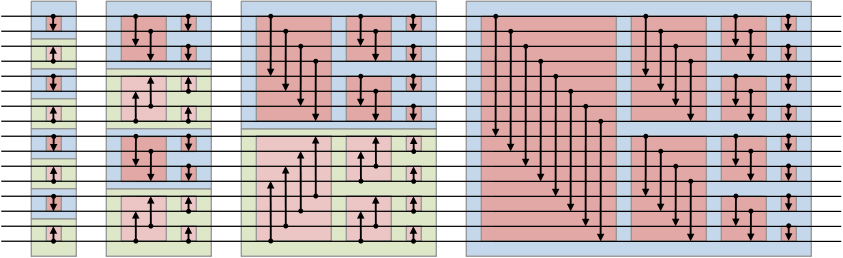
\includegraphics[width=400pt]{images/bitonic.png}
  \caption{The structure of a bitonic sorting network}
\end{figure}

% versione non potenza di 2 https://hwlang.de/algorithmen/sortieren/bitonic/oddn.htm

\section{Implementation}

The scope of the implementation is to use Numba to measure its efficiency compared to serial python algorithms and a standard CUDA C++ version.\\
The other versions are inspired by the course material and by the Wikipedia iterative implementation, with some changes to support a generic sorting direction (and of course, translated to python).\\

The Python code consists of 3 functions

\subsection{The host code}
A function named \textit{bitonic\_sort} that accepts the initial data, its size and the direction. This function loops two indices, doubling the outer one each external iteration and halfing the inner one each internal iteration.
This represents the $p=log_{2}n$ phases and $s=log_{2}p$ stages for each phase. Inside the two loops, the kernel function is called forwarding the data, the direction and passing the current phase and stage.

\subsection{The kernel code}
The \textit{global} code, called by the host and executed in the device decides which pair of elements to compare is represented by the function \textit{bitonic\_kernel}.\\
It's decorated with the \textit{@cuda.jit} decorator, that signales Numba that it's a function to compile to CUDA instructions.
This function checks if the \textbf{bitwise XOR} between the phase and the stage is bigger than the current thread global index, then executes the \textit{compare\_and\_swap} function swapping the two indices compared in the previous conditions as arguments based on if the \textbf{bitwise AND} is equal to 0 or not.

\subsection{The device code}
The last function has the purpose of swapping the elements based on their positions and the sorting direction.\\
More specifically, if the requested direction (represented by a $0-1$ valued integer) equals the direction of the two elements, the pair is swapped
This function could be further improved by adding the support for the atomic operation \textbf{Compare and Swap} \cite{cas}, that could reduce Warp Divergence by swapping conditions with mathematical calculations.

\subsection{Sequences of length not power of 2}

\section{Benchmark and Profiling}

\subsection{Environment}
The benchmark and profiling environment is represented by a computer with an AMD Ryzen 7 5800H CPU (8 Cores, 16 Threads), 16 GB of RAM and an NVIDIA GeForce RTX 3050 Ti for Laptops.
Basic specifications comprise \textbf{20 SMs} for a total of \textbf{2560 CUDA cores}, 20 RT cores and 80 Tensor cores. Clock speeds up to 1695 MHz boost at 80W, or as low as 1035 MHz for the 35W configuration, giving us quite a wide power range of 35 to 80W.
It has 4GB of GDDR6 memory on a 128-bit bus, clocked at 12 Gbps.
The \textbf{Compute Capability} Version is 8.6.

\subsection{JIT Compilation}
The CUDA runtime executes functions, called kernels, compiled for NVIDIA GPUs instruction set using the NVCC Compiler \cite{nvcc} and this is a different approach compared to Python, which is a \textbf{runtime interpreted language}.\\
To solve this issue in the fastest way without changing paradigm was to compile \textbf{Just In Time} the python kernel into machine code, \textbf{caching it} and then executing it calling the CUDA Runtime Library.
This of course comes with a delay in the first execution of a kernel (that needs to be compiled) and since the benchmarks would be cached except for the first one, the JIT compilation time has been considered separately.
On the kernel function defined for the Bitonic Sort, the compilations on the environment takes around \textbf{0.3 seconds}, so it's noticeable if you want to compare with a sequential approach or a CUDA C version with a cold start.

\subsection{Serial and Parallel approach}

The first benchmark is between two serial approaches and the Numba implementation, with all three being in Python.\\
To have some meaningful data, the benchmark had multiple size of the array, starting from $n=2^8$ to $n=2^14$, doubling each time.\\
As we can see from the following image, the Numba implementation time maintains a negligible time while both the recursive and iterative serial approaches went above the second for the last one, with the recursive being slight better.\\
This has to be expected since the parallel version is ideally $O(log(n)^2)$ on each core, so noticeably faster than a sequential version. This is of course not completely true in reality since the GPU has not an infinite number of cores and with a further increase on the input size we'll see in the next section a rapid increase on time, but still slower than the serial version.

\begin{figure}[H]
  %\centering
  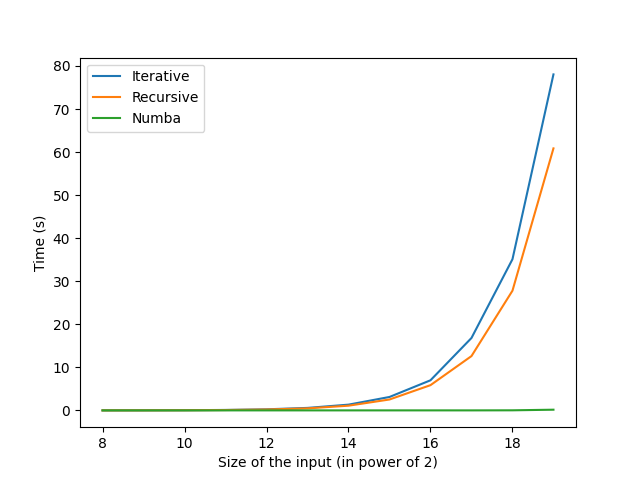
\includegraphics[width=400pt]{images/cpu_vs_gpu.png}
  \caption{Time comparison between different implementations}
\end{figure}

The following table shows in details the results for each size

\begin{center}
  \begin{tabular}{ |c|c|c|c| }
    \hline
    \textbf{Size (Power of 2)} & \textbf{CPU Recursive} & \textbf{CPU Iterative} & \textbf{GPU} \\
    \hline
    8                          & 10 ms                  & 10 ms                  & 10 ms        \\
    9                          & 10 ms                  & 10 ms                  & 10 ms        \\
    10                         & 10 ms                  & 10 ms                  & 10 ms        \\
    11                         & 10 ms                  & 10 ms                  & 10 ms        \\
    12                         & 10 ms                  & 10 ms                  & 10 ms        \\
    13                         & 10 ms                  & 10 ms                  & 10 ms        \\
    14                         & 10 ms                  & 10 ms                  & 10 ms        \\
    15                         & 10 ms                  & 10 ms                  & 10 ms        \\
    16                         & 10 ms                  & 10 ms                  & 10 ms        \\
    17                         & 10 ms                  & 10 ms                  & 10 ms        \\
    18                         & 10 ms                  & 10 ms                  & 10 ms        \\
    19                         & 10 ms                  & 10 ms                  & 10 ms        \\
    \hline
  \end{tabular}
\end{center}

\subsection{CUDA C and Numba}

The second and last benchmark compares the Numba and Python implementation with the CUDA C one.\\
The code is basically the same but in different languages, so the theoretical performances should be the same.
As we can see from the image below, the CUDA C implementation, while it's faster, it is just for a constant coefficient.\\
This means that there's an overhead, probably result of the Python runtime and the Numba abstraction layer, that makes the CUDA C implementation around 3 times faster.\\
While this seems a huge number in performances, given the fact that its constant it can be an acceptable difference in many cases when someone would prefer the faster development time that Python allows.

\begin{figure}[H]
  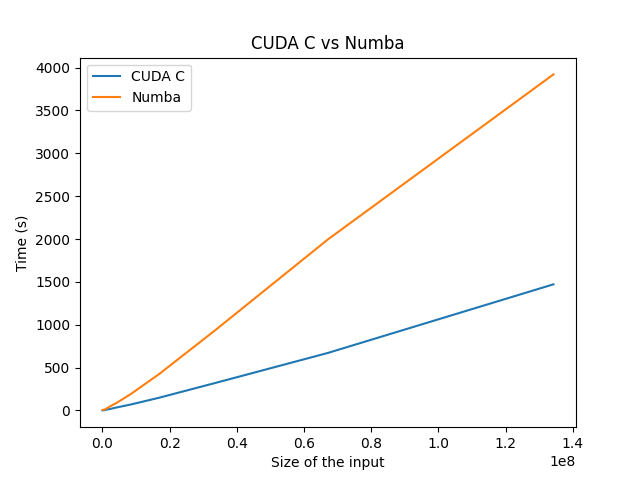
\includegraphics[width=400pt]{images/cpp_vs_py_2.png}
  \caption{Time comparison between parallel implementations on different platforms}
\end{figure}

The last figure shows the same results but making the data extrapolation easier showing the values on a power of 2 scale

\begin{figure}[H]
  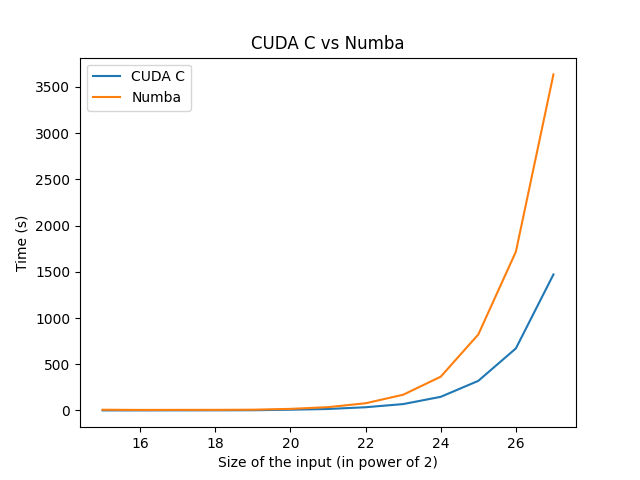
\includegraphics[width=400pt]{images/cpp_vs_py.png}
  \caption{Time comparison between parallel implementations on different platforms with better value/time visualization}
\end{figure}

The last table of the section again shows the detailed results

\begin{center}
  \begin{tabular}{ |c|c|c|c| }
    \hline
    \textbf{Size (Power of 2)} & \textbf{Cuda C++} & \textbf{Python Numba} \\
    \hline
    15                         & 10 ms             & 10 ms                 \\
    16                         & 10 ms             & 10 ms                 \\
    17                         & 10 ms             & 10 ms                 \\
    18                         & 10 ms             & 10 ms                 \\
    19                         & 10 ms             & 10 ms                 \\
    20                         & 10 ms             & 10 ms                 \\
    21                         & 10 ms             & 10 ms                 \\
    22                         & 10 ms             & 10 ms                 \\
    23                         & 10 ms             & 10 ms                 \\
    24                         & 10 ms             & 10 ms                 \\
    25                         & 10 ms             & 10 ms                 \\
    26                         & 10 ms             & 10 ms                 \\
    27                         & 10 ms             & 10 ms                 \\
    \hline
  \end{tabular}
\end{center}

\subsection{Profiling Results}

Using the profiling tool $NCU$ on a kernel execution, we obtained the following results:\\

\subsubsection{GPU Speed Of Light Throughput}

\begin{center}
  \begin{tabular}{ |c|c|c| }
    \hline
    Metric Name             & Metric Unit   & Metric Value \\
    \hline
    DRAM Frequency          & cycle/nsecond & 5,75         \\
    SM Frequency            & cycle/nsecond & 1,17         \\
    Elapsed Cycles          & cycle         & 2.757.034    \\
    Memory Throughput       & \%            & 92,97        \\
    DRAM Throughput         & \%            & 92,97        \\
    Duration                & msecond       & 2,35         \\
    L1/TEX Cache Throughput & \%            & 19,44        \\
    L2 Cache Throughput     & \%            & 29,83        \\
    SM Active Cycles        & cycle         & 2.746.869,40 \\
    Compute (SM) Throughput & \%            & 16,16        \\
    \hline
  \end{tabular}
\end{center}

\subsubsection{Launch Statistics}

\begin{center}
  \begin{tabular}{ |c|c|c| }
    \hline
    Metric Name                      & Metric Unit     & Metric Value    \\
    \hline
    Block Size                       &                 & 256             \\
    Function Cache Configuration     &                 & CachePreferNone \\
    Grid Size                        &                 & 131.072         \\
    Registers Per Thread             & register/thread & 16              \\
    Shared Memory Configuration Size & Kbyte           & 8,19            \\
    Driver Shared Memory Per Block   & Kbyte/block     & 1,02            \\
    Dynamic Shared Memory Per Block  & byte/block      & 0               \\
    Static Shared Memory Per Block   & byte/block      & 0               \\
    Threads                          & thread          & 33.554.432      \\
    Waves Per SM                     &                 & 1.092,27        \\
    \hline
  \end{tabular}
\end{center}

\subsubsection{Occupancy}

\begin{center}
  \begin{tabular}{ |c|c|c| }
    \hline
    Metric Name                     & Metric Unit & Metric Value \\
    \hline
    Block Limit SM                  & block       & 16           \\
    Block Limit Registers           & block       & 16           \\
    Block Limit Shared Mem          & block       & 8            \\
    Block Limit Warps               & block       & 6            \\
    Theoretical Active Warps per SM & warp        & 48           \\
    Theoretical Occupancy           & \%          & 100          \\
    Achieved Occupancy              & \%          & 83,52        \\
    Achieved Active Warps Per SM    & warp        & 40,09        \\
    \hline
  \end{tabular}
\end{center}

\section{Conclusion}
Based on the results of this experiments, \textbf{Numba} seems a worthy framework that doesn't add too much overhead to the implementation, while having some advantages like a simpler use with the Python abstraction.\\
The difference with the C implementation is marginal and scales well and it has big improvements over the serial approach, just like one would expect from a data-indipendent algorithm.

\printbibliography

\end{document}




